% Number 880
% CAPMG  Units 
% v graph problem-solving; v bar and displacement
% KO

% Watermark
\AddToShipoutPicture*{\BackgroundPic}

\addtocounter {ProbNum} {1}

\begin{floatingfigure}[r]{.44\textwidth}
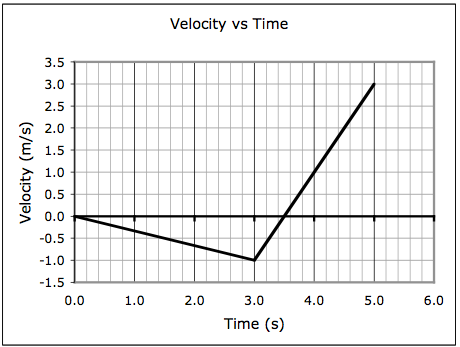
\includegraphics[scale=.54]{/Users/jgates/desktop/latex/pics/vgraph6}
\end{floatingfigure}
 
{\bf \Large{\arabic{ProbNum}}} A cart travels with the velocity shown in the graph.   \bigskip


Describe the motion in words.
\paragraph{}
\noindent
\vfill

What is the cart's displacement, in meters, during the first four seconds?
\vfill

What was the cart's average velocity over the entire five seconds of recorded motion?
\vfill

At what instant does the cart reach the farthest position in the negative direction with respect to its starting point? (Explaining your thinking might help you get the right answer and will help me help you if you�re wrong.)
\vfill

%\begin{center}
%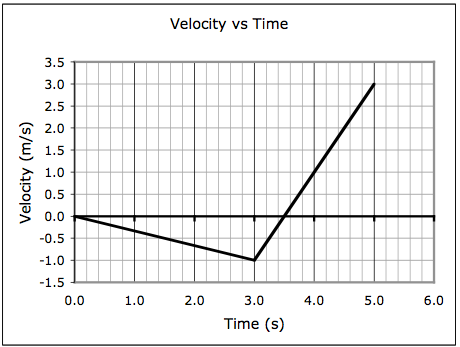
\includegraphics[scale=1]{/Users/jgates/desktop/latex/pics/vgraph6}
%\end{center}


\newpage
